\documentclass[twocolumn,linenumbers]{aastex631}
%%\documentclass[linenumbers]{aastex631}
%%\documentclass[modern]{aastex631}
%%\documentclass[twocolumn]{aastex631}
\newcommand{\vdag}{(v)^\dagger}
\newcommand\aastex{AAS\TeX}
\newcommand\latex{La\TeX}

\usepackage{mathtools, graphicx, booktabs, apjfonts, soul}
%\addbibresource{Bibliography.bib} %For bibliography

\begin{document}

\title{The Distribution of Cohesive Objects in the Universe: an Extended "Main Sequence"
\footnote{Sept, 17, 2024}}

\author[0000-0002-8482-4669]{Gabriel M Steward}
\affiliation{University of Idaho, Moscow, Idaho 83844}

\author{Matthew Hedman}
\affiliation{University of Idaho, Moscow, Idaho 83844}

\begin{abstract}

\textbf{\color{red}ABSTRACTION: this will be done last, as we need to know the end from the beginning to properly do it.\color{black}}

\end{abstract}

\keywords{KEYWORDS (111) --- KEYWORDS (112)}

\section{Introduction} \label{sec:intro}

\textbf{\color{red} [NOTE: For major notes.] \color{black}}

\textbf{\color{blue}For placeholder stuff and jotted notes. \color{black}}

The HR (Hertzsprung-Russel) diagram is a familiar sight to many. The relation of color temperature to luminosity sucinctely shows how a simple relation of two components can be used to identify, categorize, and explain objects in space. The success of the HR diagram is difficult to overstate, as it is a cornerstone of astronomy or astrophysics course. 

In recent years, a similar endeavor has been undertaken for exoplanets. Now that we have over 5000 confirmed discoveries, mass/radius plots can be constructed that show distinct domains of planetary types \citep{Chen2016, Muller2024}. These graphs, while similar in purpose and scope to the HR diagram, are not yet as successful, but likely will be in the future. One can also find similar distribution graphs for asteroids, such as mass-density plots \citep{Carry2012}. 

One may be tempted to think that these three domains of stars, exoplanets, and asteroids are entirely unrelated. However, that is not the case; all of them share some simple, basic properties. All of them are cohsive objects; that is, objects that are made of components in physical contact with each other, as opposed to non-cohesive objects like nebulae or galaxies. Each cohesive object has a particular mass and size, from which density and surface gravity can be determined. This means that every one of these objects can be placed on the same plot so long as two of the aforementioned values were used. 

In this paper, we present such a graph that plots the mass-density relation for all cohesive objects that we have decent measurements for, ranging from miniscule asteroids to supermassive black holes. The intention is that this plot will be shared readily among the community as a way to examine the overall distribution of objects in the universe, connecting many disciplines across astrophysics. Like the HR diagram, this distribution plot suggests many clear divisions by which to categorize objects, and even has an extended "main sequence" of sorts on which the vast majority of objects fall. 

We begin with \textbf{Results} since the primary result of this paper is the driving force behind it. \textbf{Discussion} of the distributions come next, including classification implications, outlier examinations, and uncertainties. The \textbf{Conclusion} of our work comes next, though afterward we describe the \textbf{Methods} used to gather and pair down the data. 

\section{Results} \label{sec:intro}

\begin{figure*}[htbp]
\centering
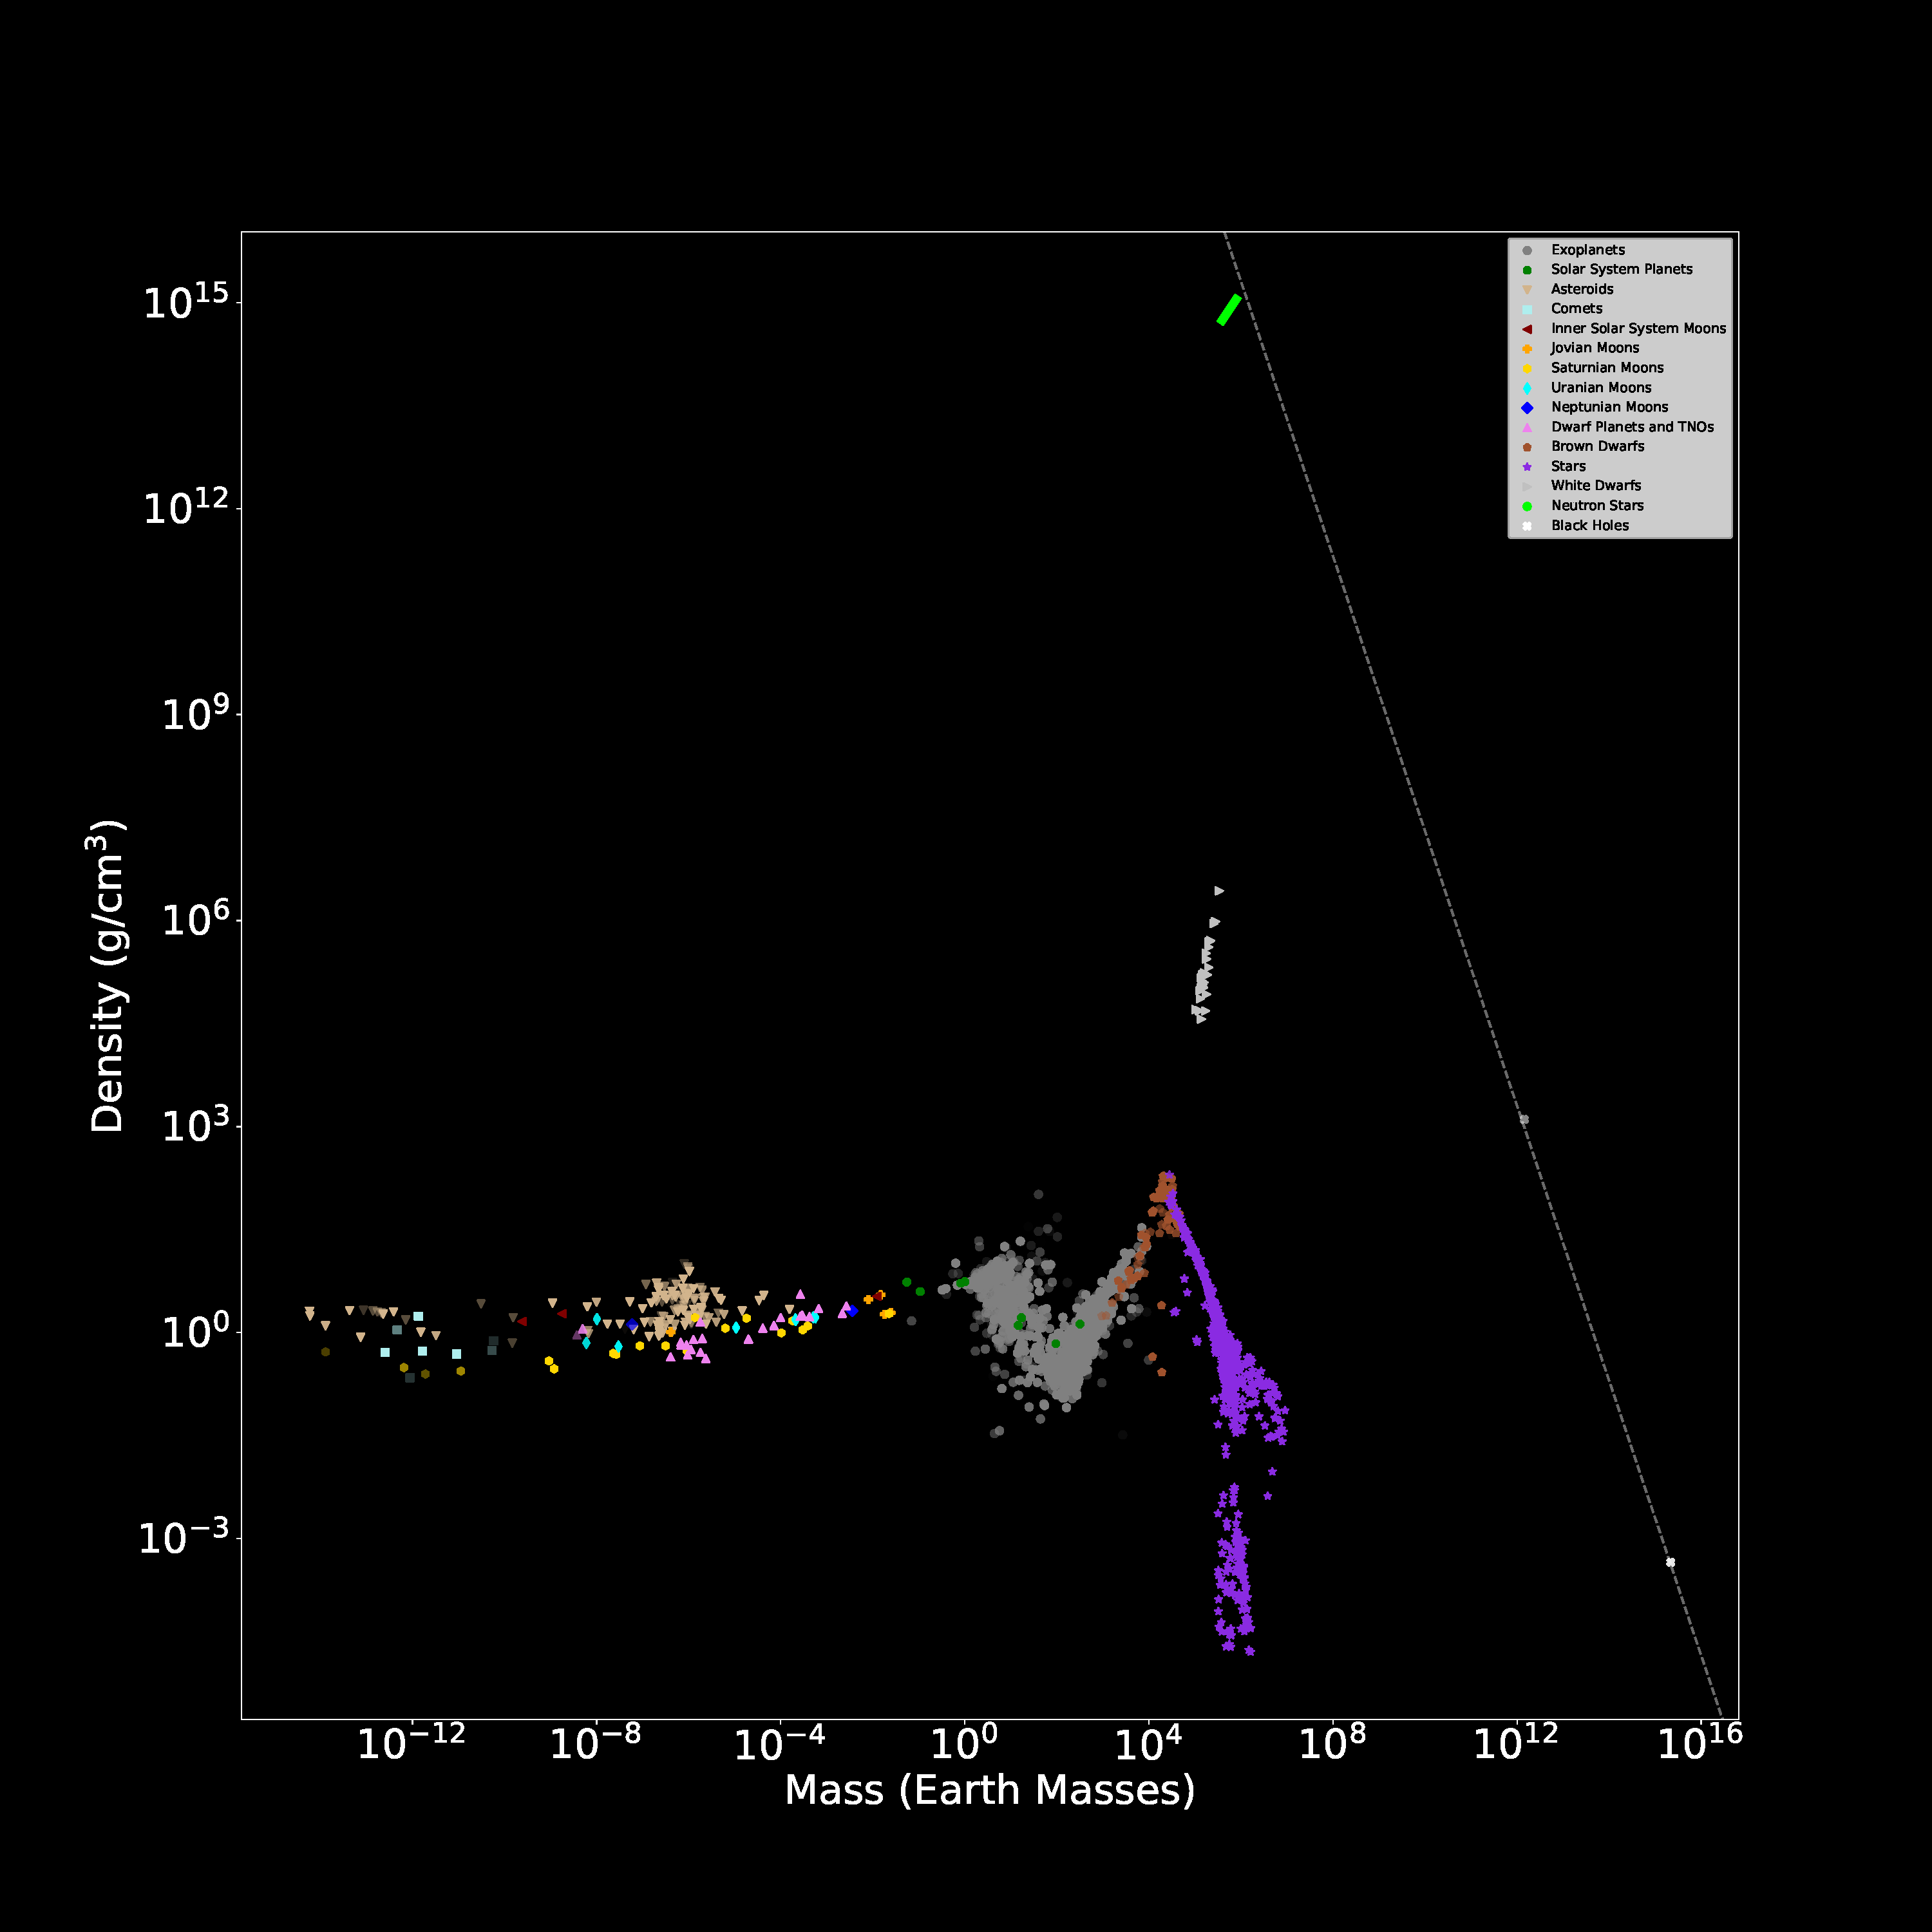
\includegraphics[scale = 0.35]{MassDensityPlot.pdf}
\centering
\caption{The relationship between density (in g/cm$^3$) and mass (in Earth masses) for cohesive objects in the universe on a log-log scale. Each kind of object is given a unique color and shape. The transparency of each point represents how large the errors are: solid objects have minimal errors while the more transparent ones have larger errors with a maximum relative permitted error of 0.5 in either mass or thrice the radius, whichever was larger for the object in question. As no  neutron star radii have been measured to precision, the general area Neutron Stars occupy is given by a green line. The dashed line represents the black hole limit, any object that reaches this line should theoretically collapse into a black hole. }
\label{fig:1}
\end{figure*}

Figure \ref{fig:1} is our primary result, showing the relation of mass and density for asteroids, comets, trans-Neptunian objects, moons, planets, brown dwarfs, stars, neutron stars, and black holes. Every data point represents a real object in the scientific literature. The points are categorized by type via shape and color, the classification assigned based on the source they were found in. This draws attention to the inconsistent distinction between exoplanets and brown dwarfs, as well of the wide vareity in exoplanets and stars. Transparency represents the relative error associated with each object: low errors plot solid points, while high errors are almost transparent. The maximum relative error plotted is 0.5 measured against the mass or volume, whichever was larger. Direct radius relative error was not used as mass correlates with radius cubed, and so the error propogations differ between the two by a factor of 3. The largest errors are particuarly noteworthy on outlier exoplanets, outlier asteroids, and particuarly small objects. 

No neutron stars have had their radii measured with sufficient precision as far as we are aware. Thus, a loose range of neutron star masses and densities are plotted as a fat line, rather than individual points. Two black hole event horizon radii have been satisfactorily measured, and they are on the plot, but to put them in contaxt we opted to plot the theoretical mass-density relation for Schwarzchild black holes.

Expanded views of various sections of Figure \ref{fig:1} are shown in Figure \ref{fig:2}, examing four different mass scales. These views make it possible to pick out individual objects among the otherwise dense clouds.  

\begin{figure*}[htbp]
\centering
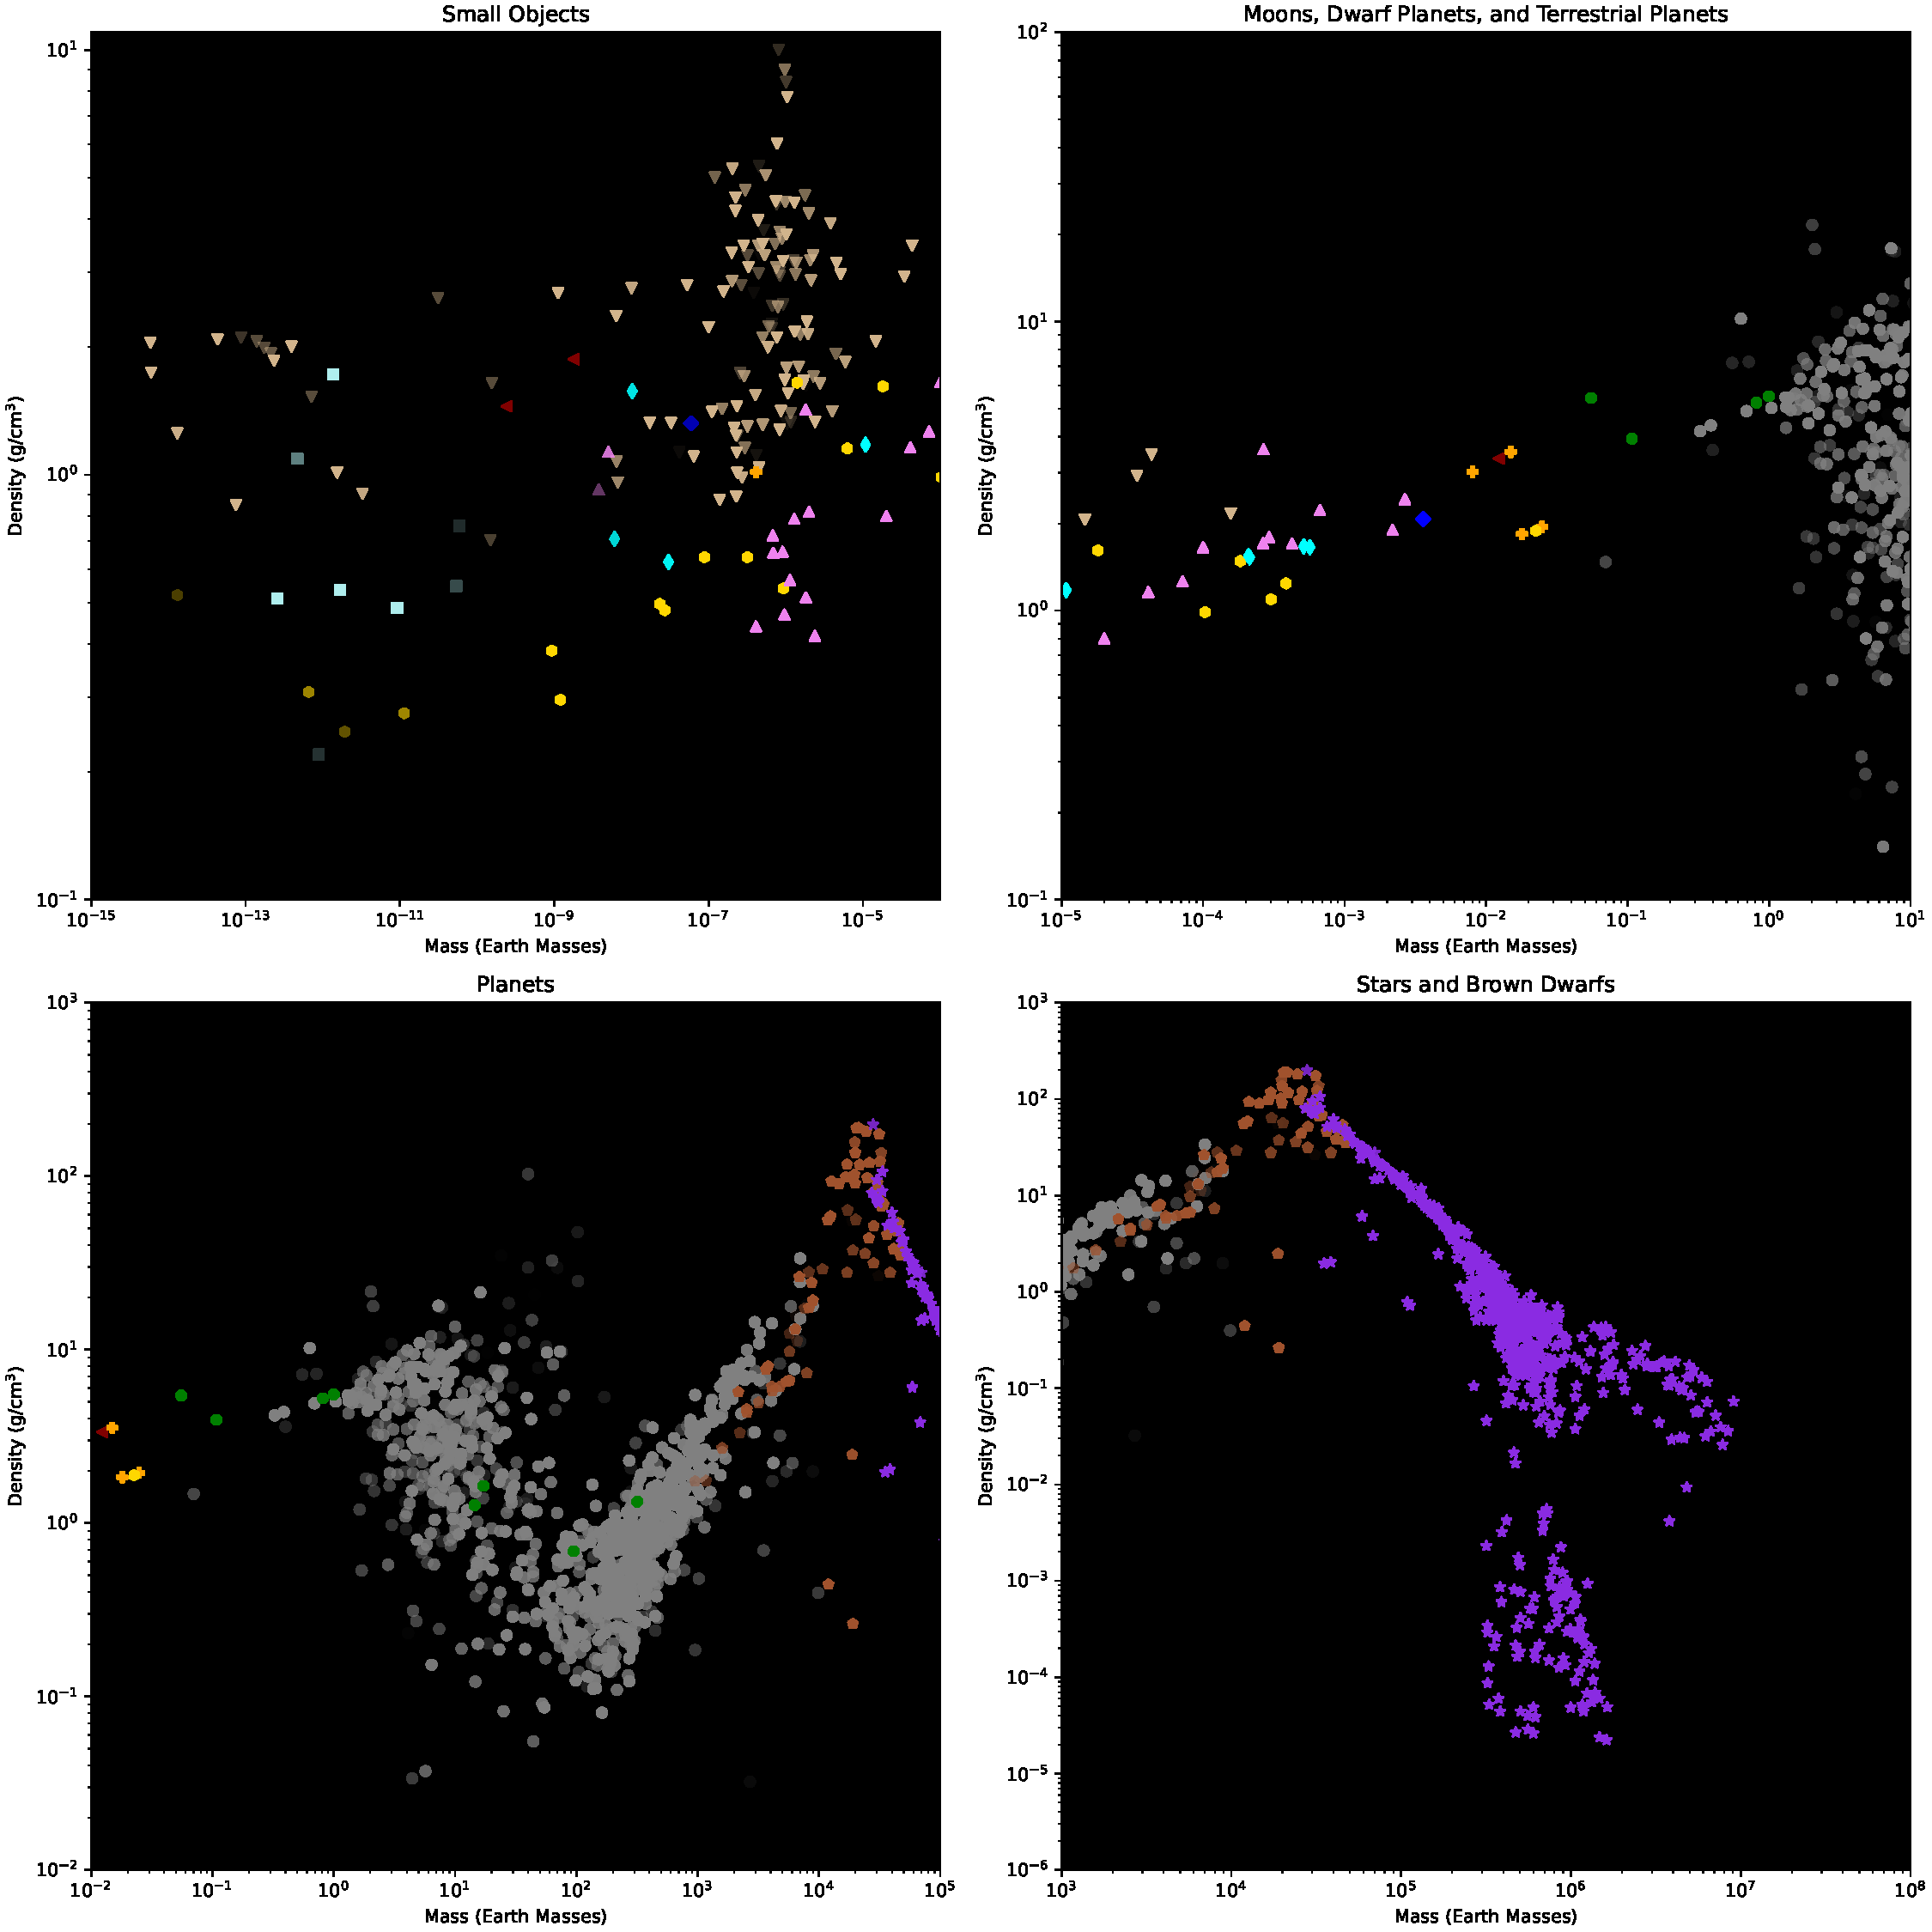
\includegraphics[scale = 0.35]{ZoomViews.pdf}
\centering
\caption{Zoomed in views of Figure \ref{fig:1} using the same colors and shapes. No view for white dwarfs or other extreme objects, as there is not much detail present in those ranges to begin with.}
\label{fig:2}
\end{figure*}

The actual data collected in our dataset are mass and radius, not mass and density. Mass and density were chosen for Figure \ref{fig:1} because it makes it easier to see distinct categories of objects, particuarly in the lower-mass regime of exoplanets. However, the mass-radius relation is not ignored; we have it plotted in Figure \ref{fig:3} alongside other combinations of mass, radius, density, and surface gravity. 

\begin{figure*}[htbp]
\centering
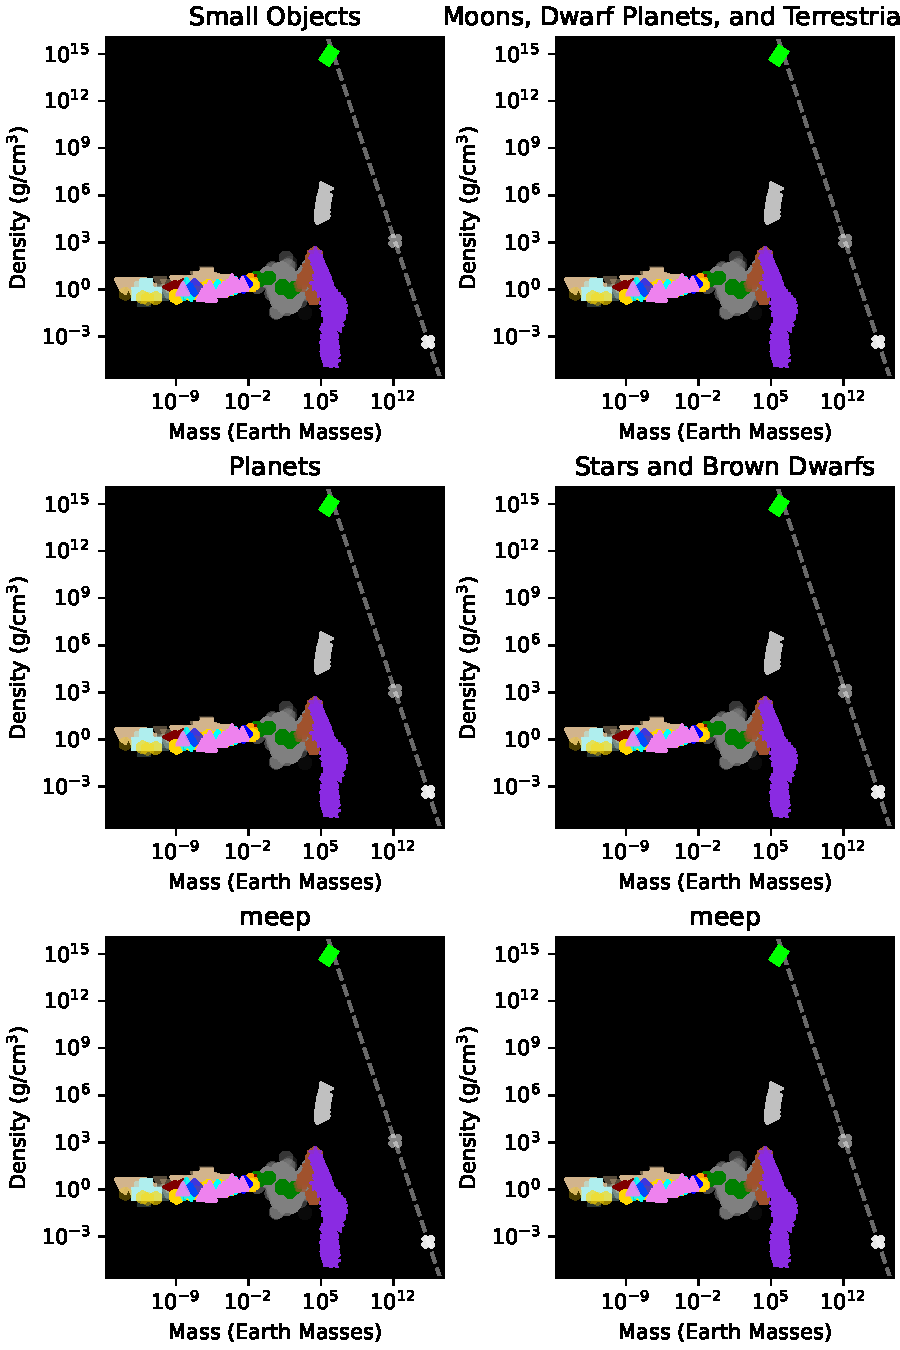
\includegraphics[scale = 1]{AltVariableViews.pdf}
\centering
\caption{Alternate views of the data set showing different combinations of mass, radius, density, and surface gravity. Colors and shapes are identical to  Figure \ref{fig:1}.}
\label{fig:3}
\end{figure*}

\section{Discussion} \label{sec:intro}

Each individual area of Figure \ref{fig:1} reveals trends in the distribution of objects in the universe, though most of these smaller-scale trends have been noted by those studying those scales. As a whole, however, this graph showcases a seemingly unbroken progression from the smallest asteroids to the largest blue stars, cutting through most other kinds of objects along the way. In the same sense that stars have a "main sequence" along which most of them lie, cohesive objects have an "extended main sequence" that contains the stellar one as the largest regime. Of the objects considered here, only compact objects, giant stars, supergiant stars, and certain actively collapsing bodies clearly lie off this extended main sequence. 

One might be tempted to describe this extended main sequence as an evolution of how objects develop the more mass they accrete, but this should be avoided. Stars form from clouds of gas, and have formed since before there were enough heavy elements to even make asteroids. One does not keep throwing asteroids at each other until fusion begins in nature. What this extended main sequence does show is that nature tends to form objects of certain masses out of certain materials, and that when objects get massive enough they tend to smoothly transition into another kind of object. Asteroid-like objects do accumulate in to terrestrial planets over time. Once terrestrial planets accumulate enough mass they will begin to accrete more volatile materials and become ice (or volatile) giants (), and the same goes for the transition to gas giants. One can imagine preferential accretion of heavy materials over volatile ones to get particuarly massive terrestrial palnets, and there are a handful of objects like this, but such "ovedense worlds" are rare (), and there do not appear to be any in the mass regime of gas giants. Gas giants will transision to stars once hydrogen fusion begins at a very well known point, and then at this point the extended main sequence ends with the most massive stars that are stable. Perhaps population III stars would extend it further, but we have not conclusively observed them (). 

Another reason to avoid treating the extended main sequence as a sequence of development is that small objects can be created from larger ones. Many asteroids are fragments of once larger bodies, and terrestrial planets could have had extensive hydrogen envelopes in the past that were blown off over time (). Formation pathways for objects of the same class can vary: the largest gas giants could either form in a circumstellar disc or directly from a stellar nursery (). The extended main sequence is more of an examination of what kinds of objects can exist. There are no rocky bodies the size of Jupiter. There are no gaseous objects the size of asteroids. And nothing less massive than a star is burning any hydrogen. (Human activities excepted).  

There are a handful of objects not on the extended main sequence. Naturally, there are the giant and supergiant stars that were deviations from the original main sequence in the first place, stars approaching the ends of their lives as they run out of hydrogen to burn. The stellar remnants--white dwarfs, neutron stars, and black holes--are also not on the extended main sequence, and the jarring lack of objects connecting these regimes is indicative of the dramatic processes that form them. (Though notably the difference between the smallest black holes and neutron stars is not very large ()). There is no "gradient" to becoming a compact object. 

The only other distinct class of object clearly off the extended main sequence are collapsing objects: very young stars, brown dwarfs, and gas giants that are inflated due to their recent formation (). We do not have many of these objects plotted as we have measured so few of them, much like there are not many stars measured that are in the process of moving onto the supergiant stage of their lives. They simply do not spend enough time in these regimes for there to be a large population. 

Examining the distribution at smaller scales now, we can identify specific trends. The first such trend is merely an illusion: there are very few tiny objects plotted, but a large number after about 10e-8 Earth masses. This is not a real difference, there are far more tiny objects in the Solar System than there are larger ones (), this is merely an observation bias since larger objects are easier to see. Many of the smallest objects plotted were visited by spacecraft, including the smallest, Itokawa ().  

The majority of plotted asteroids cluster around 10e-6 Earth masses, and here we can see a distinct difference between rocky objects and icy objects. The asteroids have generally larger densities than the trans-Neptunian objects and icy Saturnian moons. This is due largely to their material: ices are less dense than rock (). The densest of asteroids are likely errors in measurement or reporting, as their density is slightly higher than that of pure iron (). That said, there are no doubt some true metallic meteorites out there, due to fragmentation of a differentiated body (). 

At the tail end of the cluster of asteroids, we reach the first object gravitationally rounded in a normal manner, Saturn's moon Mimas (), marking the beginning of objects that are rounded. The largest irregular object, Vesta, is the second most massive asteroid, marking the point at which there are no more irregular objects (). These two objects only differ in mass by a single order of magnitude, but they nonetheless mark the change between irregular and spherical objects. This change conicides with a pecular trend: the range of densities between objects begins to narrow at this point. There are no very dense asteroids of this size, but also no icy objects with particuarly low densities. The trend appears vaguely linear. This has been noticed before (). While it is somewhat sensible that no solid iron object could be this large without extreme circumstnaces, the lack of low-density icy objects is unusual, for ice itself should not compress this much (). 

With this, we reach the point in the plot with the least information, the realm of the largest dwarf planets, major moons of the solar system, and the smallest planets. Pluto, Eris, and Triton cluster together, evidence of their common origin (). Io, Europa, and the Moon all fall in a line, for they are largely rocky bodies, while Titan, Gannymede, and Callisto are in a separate less dense line, being icy bodies. Mercury and Mars sit alone with few neighbors. After all, we are only now reaching the sensitivity required to dettect these objects, and most exoplanet candidates did not pass through the error requirements. 

Extrapolation can still teach us about the smallest of planets, however. Mars clearly lies in-line with the larger Venus, Earth, and terrestrial exoplanets. Mercury does not, but it is well known that its density and metal content are unusually high (). It remains to be seen if such particuarly dense small planets are regularly created in the universe, or if Mercury is truly an outlier. 

The observed densities of exoplanets near Earth in mass do not vary all that much, but once a planet reaches a few earth masses, there is a far larger variety of densities it can take. We have now reached the boundary between terrestrial planets and volatile planets (also known as the ice giants). This is the least defined area of the extended main sequence. It is decidedly unclear where rocky worlds end and volatile worlds begin. There are even a handful of "overdense" worlds, some more massive than Uranus and Neptune, that have densities that imply a potentially rocky composition (). There is also indication that there are a handful of "water worlds" that exist in this region (), a type of planet that is neither terrestrial nor volatile--at least not in the same sense that Uranus and Neptune are volatile. The unfortunate reality is that planets in this uncertain range are the most common type of planet in the univesre (), and we are unfortuante enough not to have any examples of a planet in this regime within our own solar system. The true nature of this regime may remain mysterious for many more years. However, for all we cannot say about this region, we can say that it is continuous, and does not break off the extended main sequence in any significant manner. It merely has a wide variety within the sequence. 

The boundary between volatile planets and gas giants is a bit easier to define, as there is a clear distinction between the higher mass/lower density trend of volatile planets and the higher mass/higher density trend of gas giants. It just so happens that Saturn sits keenly in the middle of these two trends, indicating that it is one of the smallest gas giants possible (). Below Saturn on the plot are a handful of volatile planets and gas giants that are underdense--the so-called "puffballs" that are inflated due to their proximity to their host stars (). 

Jupiter is a bog-standard example of a gas giant, right in the middle of lots of others found in the univesre. As gas giants get more massive, they become denser on a rleatively predicrable trajectory until they reach the masses required to start hydrogen fusion, and thus become stars (). This leads us into the question of brown dwarfs: no matter which values are plotted, be they mass, radius, density, or surface gravity, there is no clear distinction between gas giants and brown dwarfs. They are only colored differently on the plot because of the sources they were drawn from, and there is a large overlap between the two classifications. From this, we see no reason to differentiate the two objects from each other, except possibly through formation pathway, but there is not a clear way to determine the method by which an object formed. Some have suggested the deuterium fusion limit as a differentiator (), but we see no indication of that influencing the object on a large scale. 

Stars follow the familiar pathways of the HR diagram, though they appear different when mass and density are considered. The trend of main sequence stars is higher mass, lower density. Low mass stars have little variation in density, while high mass stars show larger variability. The Sun is a completely normal member of the main sequence. The giant branch breaks off from the main sequence at masses around that of the sun, and points toward the disconnected supergiant region. This area contains the least dense objects in the universe--even less dense than supermassive black holes! 

Black holes and the other compact objects are off the extended main sequence and do not have as many clear relations with the other objects. That said, the distribution of white dwarfs does clearly point away from the stars and toward neutron stars in a sort of tenuous link. Strictly speaking, it may not be appropriate to call the event horizon radius of a black hole its "size," but as the interior of a black hole is unknown that is surely the size they appear to be. \textbf{\color{red}[(Is it important to mention apparent horizons?)]\color{black}}

There are no doubt many objects missing from consideration. There are no doubt many smaller asteroids, but plotting the tiny grains we have sampled of this size distribution would just needlessly extend the graph without any general benefit. Tiny planets and exomoons certainly exist, we just have not observed them. We also need to consider the fact that our solar system may give us a biased sample of certain objects; it is possible our moons and dwarf planets are not typical, or that many systems simply won't have iron asteroids, or that the trend of heaveir icy objects being denser is not one that exists elsewhere. 

Despite these holes, the continuous connection between all the cohesive objects on the extended main sequence is clear. The universe is interconnected across all scales. This includes scales not presented on this graph: interstellar dust can be single atoms, or it can include little bits that coalesce over time into asteroid sized objects (). While there may be some unusually large objects out there, the extended main sequence does appear to end with the most massive of stars, and no cohesive object could ever be larger than a black hole. At that point we are forced to admit that the universe has no cohesive objects, merely collections of these objects, such as galaxies. Whether a similar "sequence" can be found for these objects, connecting nebula to galaxies, is beyond the scope of this paper. 

\section{Conclusion} \label{sec:intro}

\textbf{\color{blue}CONCLUSION: Discuss the major points, how the graph might be used, and what we can learn from it. Also note holes in the graph that could be filled in the future. \color{black}}

\section{Methods} \label{sec:methods}

The data for cohesive objects was gathered from a large number of sources, tabulated in \textbf{\color{red}BELOW TABLE\color{black}}. To be considered for the final data set, the most basic requirements were a mass measurement and a radius measurement with reported errors. Sometimes these values would come from entirely different sources, so a lot of searching for missing values was involved. At times, mass and radius were not reported with errors, but a value like density was, so we could calculate backward. At this early stage in information collection, data was judged by eye if it was good or bad, with a lot of data simply ignored for low certainty or precision or if the source was suspect. 

After all the data points were collected, we began to pair them down. 

Minimum neutron star \citep{Suwa2018}. 

Maximum neutron star \citep{Romani2022}. 

Neutron star radius \citep{Ozel2016}. 

TNO Test \citep{Brown2017}. 

TEST \citep{Morin2010}

\textbf{\color{blue}METHODS: In the back discuss the nitty-gritty deatils of where the data was gathered from, how it was trimmed down, and what the requirements were. Also discuss outlier handling. This is mainly where a ton of citaitons are going to go. \color{black}}

\begin{acknowledgments}
Insert ACK here. 

\textbf{\color{blue}Data availability? Would like to make it clear that we'll give all the information after just being asked...\color{black}}

\textbf{\color{red}[Not sure who needs to be put here who won't be put on the author list. Though there is going to be funding recongition here.]\color{black}}
\end{acknowledgments}

\appendix

\section{Appendix?}

Appendix!

\bibliography{Bibliography}{}
\bibliographystyle{aasjournal}

\end{document}